\documentclass[11pt,a4paper]{article}

\usepackage[T1]{fontenc}
\usepackage[utf8]{inputenc}
\usepackage[french]{babel}
\usepackage{geometry}
\usepackage{enumitem}
\usepackage{amsmath}
\usepackage{graphicx}
\usepackage{float}
\usepackage{booktabs}
\usepackage{hyperref}

\geometry{margin=2.5cm}

\hypersetup{
    colorlinks=true,
    linkcolor=blue,
    urlcolor=blue
}

\title{Projet --- Analyse de la Polarisation\\\large Rapport d'avancement --- Phase 2}
\author{}
\date{\today}

\begin{document}

\maketitle

\section{Objectif de cette phase}

Cette deuxi\`eme phase avait un objectif tr\`es concret : faire passer le projet d'une base de code ex\'ecutable \`a une version plus propre, plus coh\'erente avec le sujet, et capable de produire de premiers r\'esultats exp\'erimentaux exploitables dans le futur rapport final.

Plus pr\'ecis\'ement, cette phase visait \`a :
\begin{itemize}[leftmargin=*]
    \item stabiliser la cha\^\i ne de calcul de la mesure \(\phi_2\) ;
    \item enrichir la documentation interne du code ;
    \item renforcer la v\'erification automatique par tests ;
    \item g\'en\'erer des premiers graphiques pour les questions exp\'erimentales.
\end{itemize}

\section{Rappel de l'\'etat de d\'epart}

Au d\'ebut de cette phase, le projet disposait d\'ej\`a :
\begin{itemize}[leftmargin=*]
    \item d'une structure de code modulaire ;
    \item de g\'en\'erateurs de profils approval et ranking ;
    \item d'une premi\`ere version des distances de Hamming et de Spearman ;
    \item d'une premi\`ere version de \(\phi_2\), \(u_1\), \(\widetilde{u_2}\), \(\phi_{d_H}\) et \(\phi_{d_S}\) ;
    \item d'un petit jeu de tests unitaires.
\end{itemize}

Cependant, plusieurs parties \'etaient encore explicitement provisoires, en particulier la partie \(\phi_2\), qui avait une version pragmatique mais pas encore strictement align\'ee avec la d\'efinition du PDF.

\section{Nouveaut\'es et am\'eliorations de la phase 2}

\subsection{Correction de la d\'efinition de \texorpdfstring{$d^{c_k,c_l}(p)$}{d(k,l)}}

Le changement principal de cette phase concerne le calcul des quantit\'es interm\'ediaires utilis\'ees dans la mesure \(\phi_2\).

Le sujet d\'efinit :
\[
n_{c_kc_l}(p)
\]
comme le nombre de votantes qui pr\'ef\`erent \(c_k\) \`a \(c_l\), puis :
\[
d^{c_k,c_l}(p)=\left|n_{c_kc_l}(p)-n_{c_lc_k}(p)\right|.
\]

La premi\`ere version du code utilisait une autre agr\'egation, suffisante pour lancer les premiers essais mais incorrecte vis-\`a-vis de la d\'efinition exacte du sujet.

Cette partie a donc \'et\'e corrig\'ee dans :
\begin{itemize}[leftmargin=*]
    \item \texttt{src/pairwise.py}
\end{itemize}

\paragraph{Cas approval}
On compte maintenant :
\begin{itemize}[leftmargin=*]
    \item \(n_{c_kc_l}(p)\) comme le nombre de votantes telles que \(a[k]=1\) et \(a[l]=0\) ;
    \item \(n_{c_lc_k}(p)\) comme le nombre de votantes telles que \(a[l]=1\) et \(a[k]=0\).
\end{itemize}

\paragraph{Cas ranking}
On compte maintenant :
\begin{itemize}[leftmargin=*]
    \item \(n_{c_kc_l}(p)\) comme le nombre de votantes classant \(c_k\) devant \(c_l\) ;
    \item \(n_{c_lc_k}(p)\) comme le nombre de votantes classant \(c_l\) devant \(c_k\).
\end{itemize}

Dans les deux cas, la quantit\'e stock\'ee dans le code est bien :
\[
\left|n_{c_kc_l}(p)-n_{c_lc_k}(p)\right|.
\]

\subsection{Correction de la formule de \texorpdfstring{$\phi_2$}{phi2}}

Une fois \(d^{c_k,c_l}(p)\) corrig\'ee, la formule d'agr\'egation de \(\phi_2\) a elle aussi \'et\'e mise en coh\'erence avec le sujet.

Le code utilise maintenant l'agr\'egation :
\[
\phi_2(p)=\sum_{\{c_k,c_l\}\in C^2}\frac{n-d^{c_k,c_l}(p)}{n\binom{m}{2}}.
\]

Cette correction a \'et\'e appliqu\'ee dans :
\begin{itemize}[leftmargin=*]
    \item \texttt{src/phi2.py}
\end{itemize}

Cette modification est importante car elle change le sens de la mesure :
\begin{itemize}[leftmargin=*]
    \item si toutes les votantes ont la m\^eme pr\'ef\'erence entre deux candidates, alors \(d^{c_k,c_l}(p)=n\) et la contribution vaut \(0\) ;
    \item si le profil est parfaitement coup\'e en deux blocs oppos\'es sur cette paire, alors \(d^{c_k,c_l}(p)=0\) et la contribution vaut son maximum.
\end{itemize}

\subsection{Ajout de commentaires pour la soutenance}

Les fonctions principales ont \'et\'e annot\'ees avec des commentaires de documentation plus explicites.

Le but n'\'etait pas seulement d'expliquer le code, mais surtout de rendre visible :
\begin{itemize}[leftmargin=*]
    \item la fonction de chaque bloc ;
    \item son lien avec une question du sujet ;
    \item les d\'ependances entre modules.
\end{itemize}

Des commentaires ont \'et\'e ajout\'es notamment dans :
\begin{itemize}[leftmargin=*]
    \item \texttt{src/generation.py}
    \item \texttt{src/distances.py}
    \item \texttt{src/pairwise.py}
    \item \texttt{src/phi2.py}
    \item \texttt{src/consensus.py}
    \item \texttt{src/clustering.py}
    \item \texttt{src/measures.py}
    \item \texttt{src/experiments.py}
    \item \texttt{src/plots.py}
\end{itemize}

Cette partie est surtout utile pour la soutenance orale, car elle facilite la r\'eponse aux questions du type :
\begin{itemize}[leftmargin=*]
    \item \og cette fonction sert \`a quoi ? \fg
    \item \og elle est reli\'ee \`a quelle partie du sujet ? \fg
    \item \og quelles fonctions l'utilisent ensuite ? \fg
\end{itemize}

\subsection{Renforcement des tests}

Le jeu de tests a \'et\'e enrichi.

Auparavant, on v\'erifiait surtout :
\begin{itemize}[leftmargin=*]
    \item la forme des profils g\'en\'er\'es ;
    \item quelques propri\'et\'es simples des distances ;
    \item un cas homog\`ene pour \(\phi_2\).
\end{itemize}

Cette phase a ajout\'e des tests plus proches de la logique du sujet :
\begin{itemize}[leftmargin=*]
    \item un cas approval \`a deux candidates avec polarisation parfaite ;
    \item un cas ranking \`a deux candidates avec polarisation parfaite.
\end{itemize}

Dans ces deux cas, on v\'erifie bien que :
\[
\phi_2(p)=1.
\]

Le nombre total de tests passe ainsi \`a 9, tous valid\'es dans l'environnement courant.

\subsection{Correction de la g\'en\'eration des figures}

Les scripts d'exp\'eriences existaient d\'ej\`a, mais la g\'en\'eration des graphiques \'etait bloqu\'ee par le backend graphique de \texttt{matplotlib} dans l'environnement local.

Le probl\`eme a \'et\'e r\'esolu en configurant un backend non interactif (\texttt{Agg}) dans :
\begin{itemize}[leftmargin=*]
    \item \texttt{src/plots.py}
\end{itemize}

Cette correction permet maintenant de produire directement des fichiers \texttt{.png} sans d\'ependre d'une interface graphique install\'ee sur la machine.

\section{R\'esultats exp\'erimentaux produits durant cette phase}

\subsection{Fichiers g\'en\'er\'es}

Les scripts d'exp\'eriences ont \'et\'e ex\'ecut\'es avec succ\`es, ce qui a produit :

\begin{itemize}[leftmargin=*]
    \item des fichiers CSV dans \texttt{outputs/data/} ;
    \item des figures PNG dans \texttt{outputs/figures/}.
\end{itemize}

Les graphiques g\'en\'er\'es pendant cette phase sont :
\begin{itemize}[leftmargin=*]
    \item \texttt{phi2\_approval.png}
    \item \texttt{phi2\_ranking.png}
    \item \texttt{phidh\_approval.png}
    \item \texttt{phids\_ranking.png}
\end{itemize}

\subsection{Mesure \texorpdfstring{$\phi_2$}{phi2} pour les votes par approbation}

\begin{figure}[H]
    \centering
    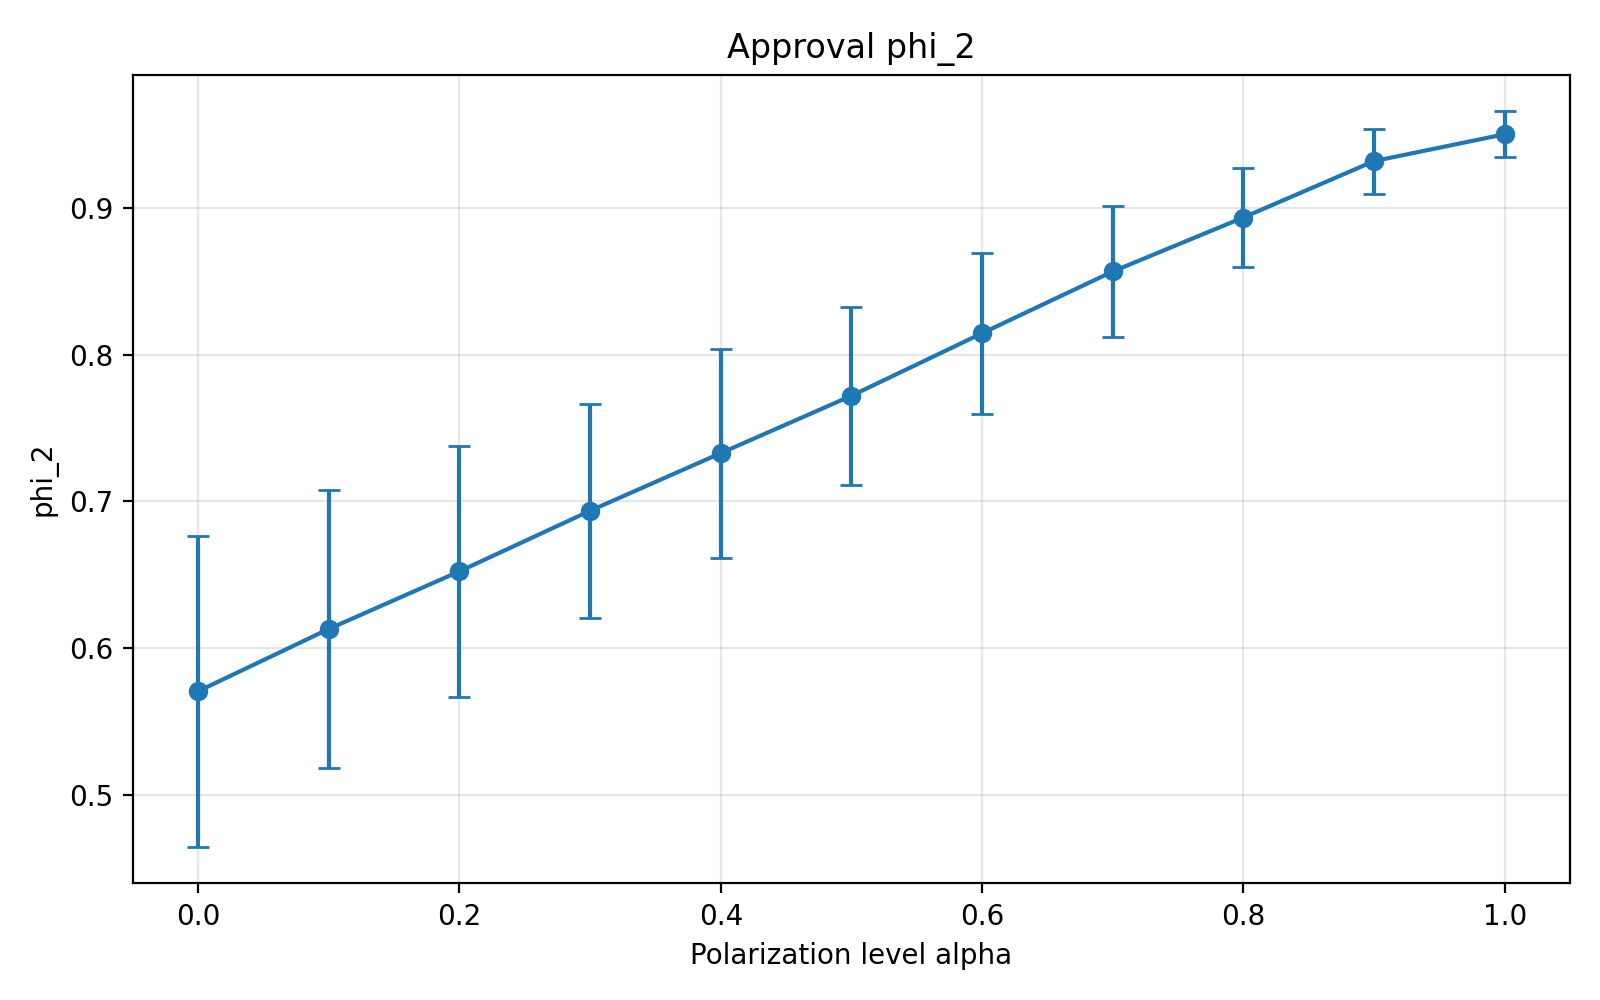
\includegraphics[width=0.82\textwidth]{../outputs/figures/phi2_approval.png}
    \caption{\'Evolution de \(\phi_2\) pour les profils approval lorsque le niveau de polarisation \(\alpha\) augmente.}
\end{figure}

Le comportement observ\'e est coh\'erent avec l'intuition du sujet :
\begin{itemize}[leftmargin=*]
    \item lorsque \(\alpha\) est faible, la mesure est plus basse ;
    \item lorsque \(\alpha\) augmente, la mesure cro\^\i t de mani\`ere r\'eguli\`ere ;
    \item pour \(\alpha = 1\), la mesure est proche de 1, ce qui correspond \`a une situation fortement polaris\'ee.
\end{itemize}

Ce graphique est particuli\`erement important car il valide \`a la fois :
\begin{itemize}[leftmargin=*]
    \item le g\'en\'erateur de profils approval ;
    \item la nouvelle d\'efinition de \(\phi_2\) ;
    \item la cha\^\i ne de calcul question 1 \(\rightarrow\) question 5 \(\rightarrow\) question 6.
\end{itemize}

\subsection{Mesure \texorpdfstring{$\phi_2$}{phi2} pour les votes par ordres totaux}

\begin{figure}[H]
    \centering
    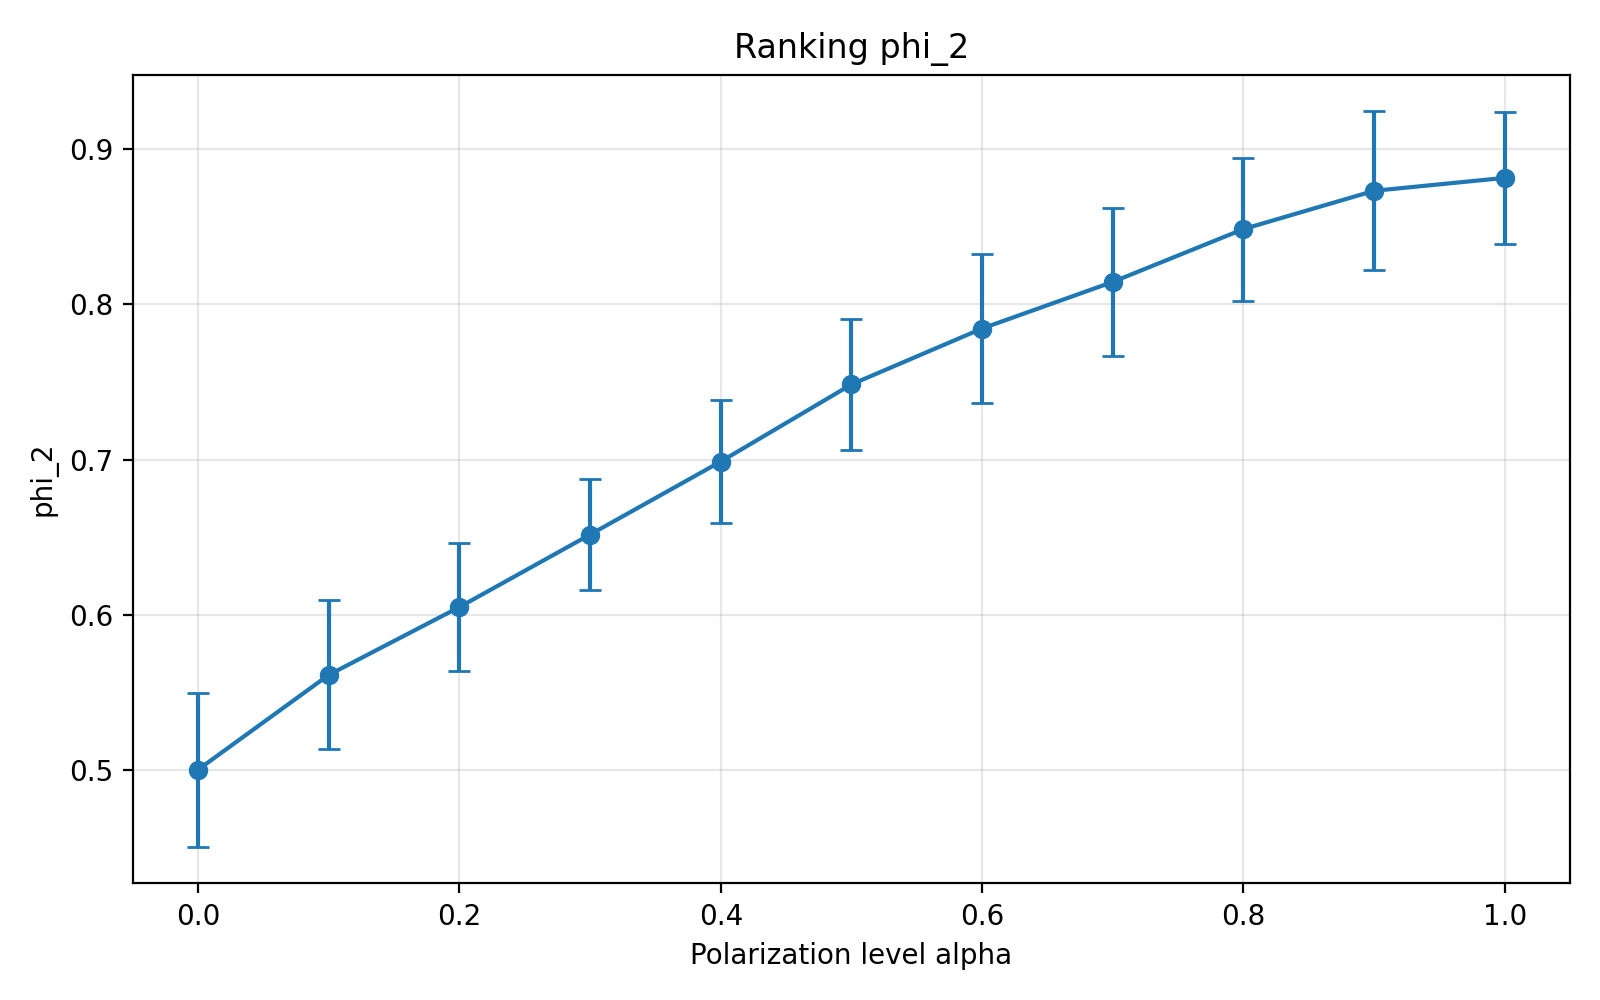
\includegraphics[width=0.82\textwidth]{../outputs/figures/phi2_ranking.png}
    \caption{\'Evolution de \(\phi_2\) pour les profils ranking lorsque le niveau de polarisation \(\alpha\) augmente.}
\end{figure}

On observe l\`a aussi une augmentation nette de la mesure avec \(\alpha\). La courbe semble un peu plus lisse et l\'eg\`erement moins extr\^eme que dans le cas approval, mais l'effet global recherch\'e est bien pr\'esent : plus la g\'en\'eration rapproche le profil de deux blocs oppos\'es, plus la mesure de polarisation augmente.

\subsection{Mesure \texorpdfstring{$\phi_{d_H}$}{phi dH} pour les votes par approbation}

\begin{figure}[H]
    \centering
    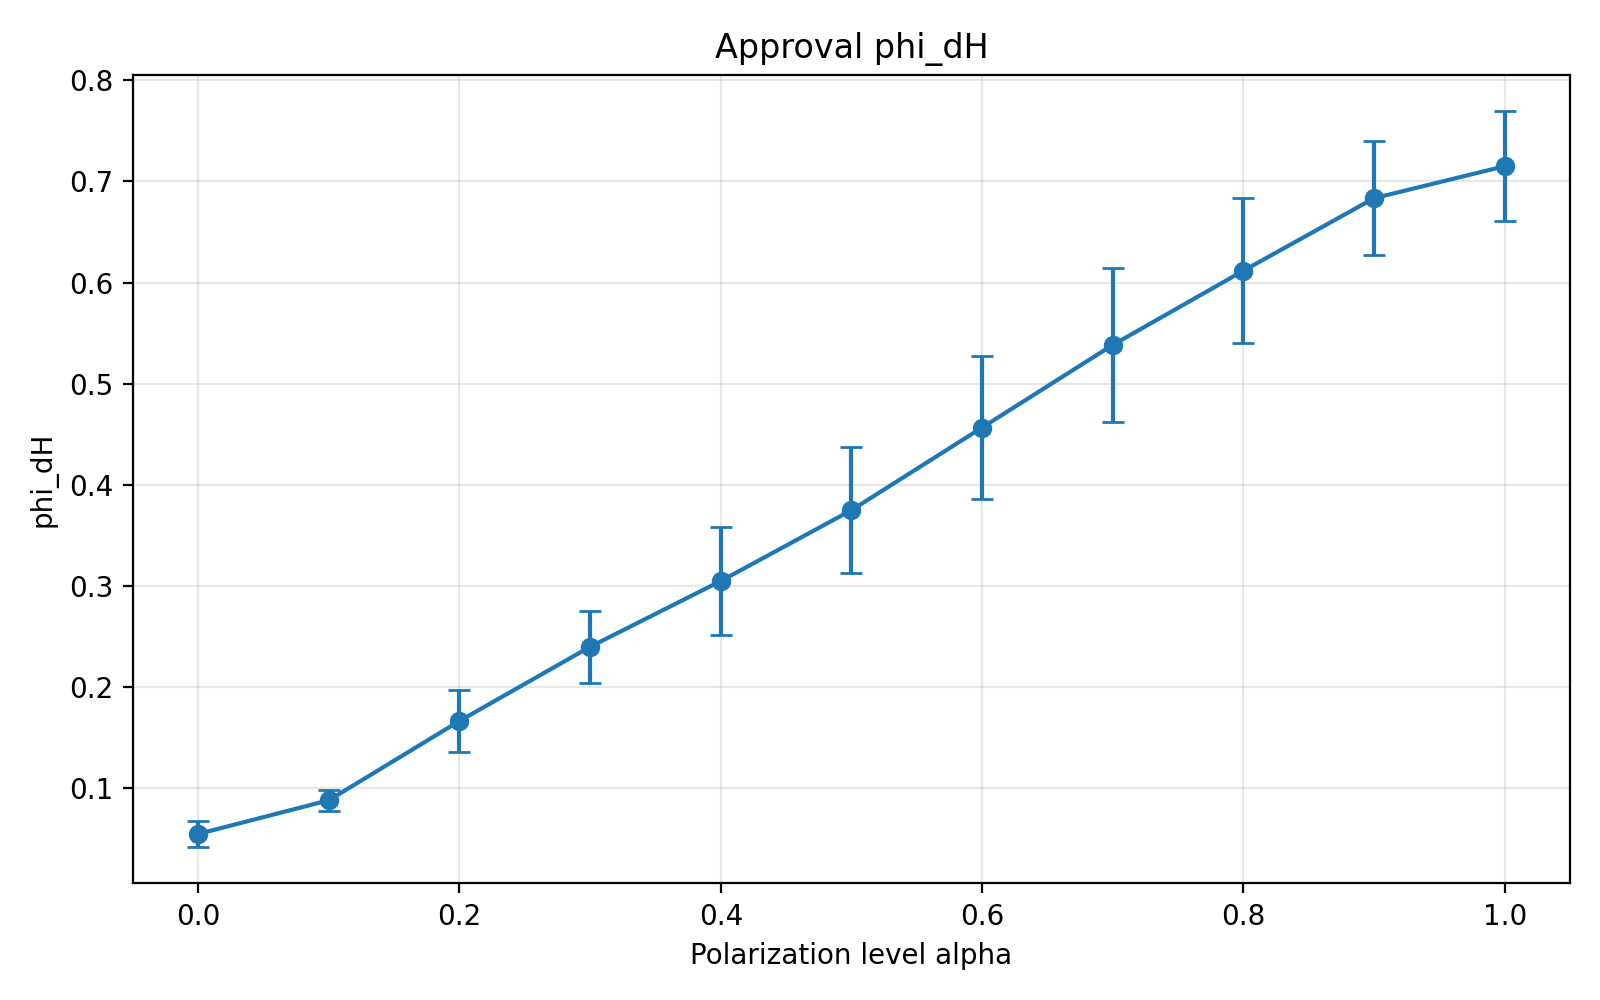
\includegraphics[width=0.82\textwidth]{../outputs/figures/phidh_approval.png}
    \caption{\'Evolution de \(\phi_{d_H}\) pour les profils approval.}
\end{figure}

La mesure \(\phi_{d_H}\) pr\'esente une croissance tr\`es claire avec \(\alpha\). C'est encourageant pour la suite, car cette mesure est construite \`a partir de :
\begin{itemize}[leftmargin=*]
    \item \(u_1\), le consensus global ;
    \item \(\widetilde{u_2}\), l'approximation \`a deux groupes obtenue par clustering.
\end{itemize}

Autrement dit, le signal obtenu semble compatible avec l'id\'ee suivante : quand le profil devient plus polaris\'e, un consensus \`a deux blocs devient beaucoup plus avantageux qu'un consensus unique.

\subsection{Mesure \texorpdfstring{$\phi_{d_S}$}{phi dS} pour les votes par ordres totaux}

\begin{figure}[H]
    \centering
    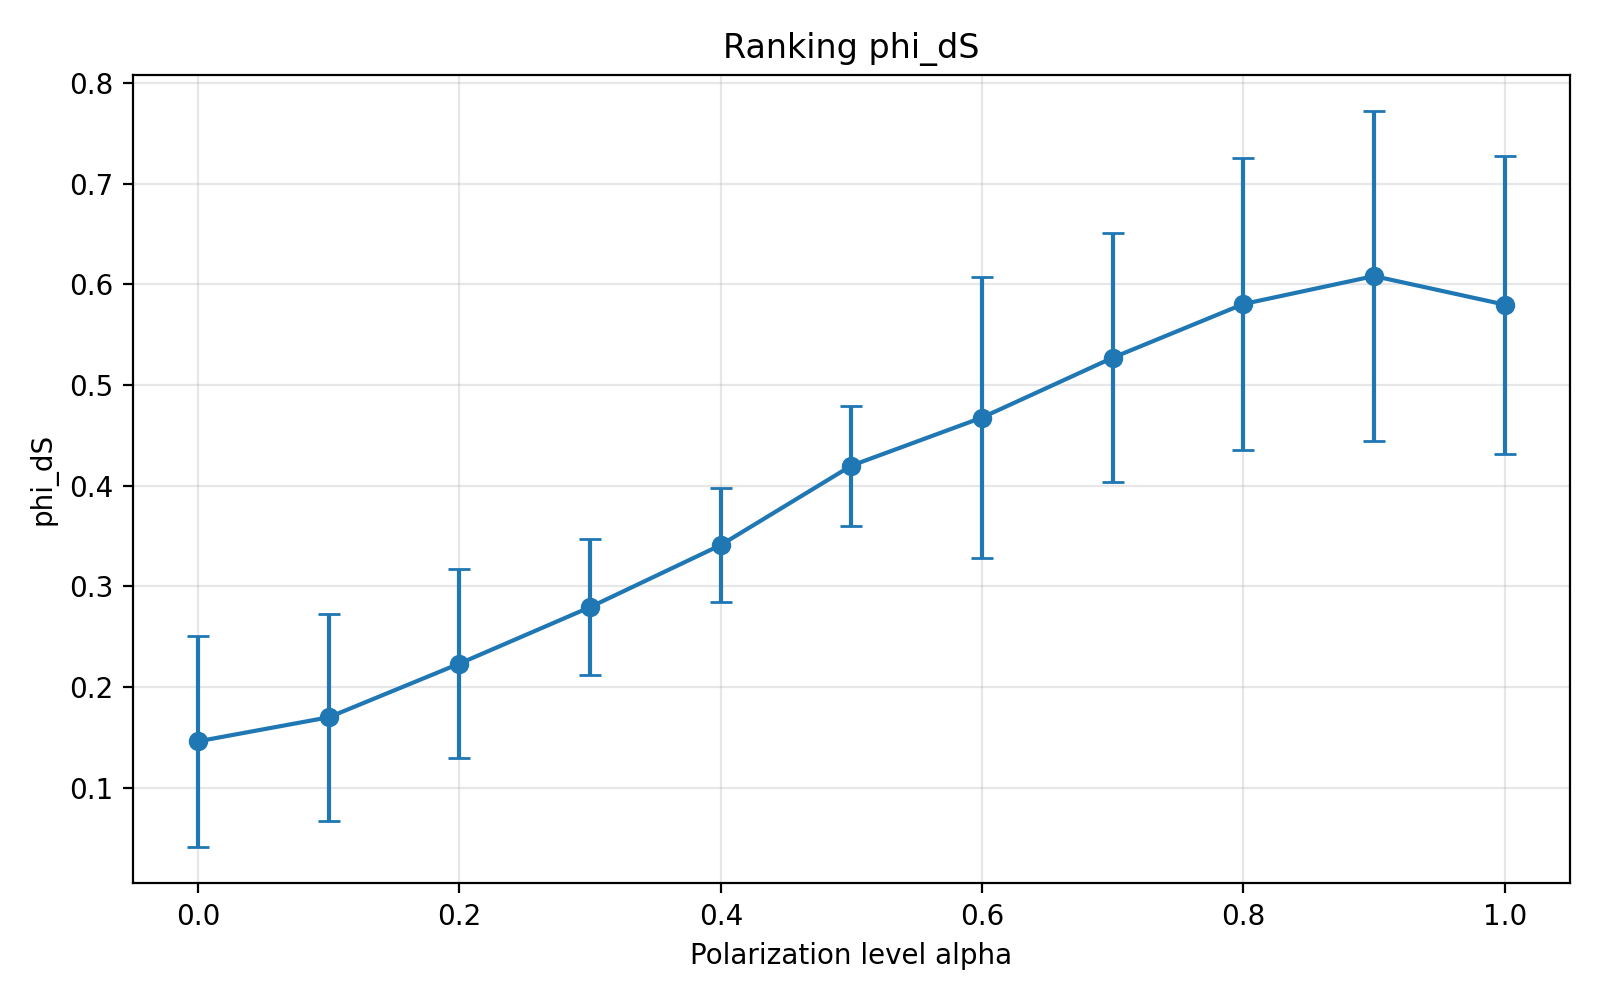
\includegraphics[width=0.82\textwidth]{../outputs/figures/phids_ranking.png}
    \caption{\'Evolution de \(\phi_{d_S}\) pour les profils ranking.}
\end{figure}

Le comportement de \(\phi_{d_S}\) est globalement croissant, mais moins stable que dans les autres graphes. Cela n'est pas surprenant, car la partie ranking repose encore sur une version de travail pour le consensus global \(u_1\), qui n'est pas encore la version finale bas\'ee sur le probl\`eme de couplage parfait de poids minimum sugg\'er\'e par le sujet.

Ce graphique reste utile, car il montre d\'ej\`a que :
\begin{itemize}[leftmargin=*]
    \item l'infrastructure exp\'erimentale fonctionne ;
    \item la mesure r\'eagit dans le bon sens ;
    \item la partie ranking doit encore \^etre raffin\'ee.
\end{itemize}

\section{Bilan technique de la phase 2}

Cette phase a apport\'e des am\'eliorations utiles \`a plusieurs niveaux.

\subsection{Ce qui a \'et\'e ajout\'e}

\begin{itemize}[leftmargin=*]
    \item de nouveaux commentaires de documentation dans les fonctions principales ;
    \item de nouveaux tests li\'es \`a la polarisation parfaite ;
    \item de nouveaux fichiers CSV de r\'esultats ;
    \item de nouvelles figures exploitables dans le rapport.
\end{itemize}

\subsection{Ce qui a \'et\'e corrig\'e}

\begin{itemize}[leftmargin=*]
    \item la d\'efinition de \(d^{c_k,c_l}(p)\) ;
    \item la formule de \(\phi_2\) ;
    \item la g\'en\'eration des figures dans l'environnement local.
\end{itemize}

\subsection{Ce qui a \'et\'e valid\'e}

\begin{itemize}[leftmargin=*]
    \item la suite de tests passe int\'egralement ;
    \item les scripts d'exp\'eriences s'ex\'ecutent ;
    \item les graphes obtenus montrent globalement une croissance de la polarisation lorsque \(\alpha\) augmente.
\end{itemize}

\section{Limites restantes}

Malgr\'e ces progr\`es, certaines parties restent provisoires.

\begin{itemize}[leftmargin=*]
    \item Le consensus ranking dans \texttt{src/consensus.py} reste une approximation par rang moyen.
    \item La partie question 11 n'est donc pas encore align\'ee avec l'indication th\'eorique du PDF.
    \item Les commentaires et graphiques produits ici servent d'abord \`a piloter le d\'eveloppement ; ils devront ensuite \^etre reformul\'es proprement dans le rapport final.
\end{itemize}

\section{Prochaine \'etape}

La prochaine \'etape logique est de se concentrer sur la partie ranking li\'ee \`a \(u_1\), car c'est le principal maillon encore fragile dans la cha\^\i ne :
\[
\text{ranking profile} \rightarrow u_1 \rightarrow \widetilde{u_2} \rightarrow \phi_{d_S}.
\]

Une fois ce point renforc\'e, il sera possible de :
\begin{itemize}[leftmargin=*]
    \item stabiliser davantage les r\'esultats de \(\phi_{d_S}\) ;
    \item pr\'eparer une version beaucoup plus proche du rendu final ;
    \item commencer la r\'edaction question par question du vrai rapport du projet.
\end{itemize}

\section{Conclusion}

Cette phase 2 a marqu\'e une vraie progression du projet. Le code n'est plus seulement une structure de d\'emarrage : il produit maintenant des mesures, des tests, des fichiers de r\'esultats et des figures. La correction de \(\phi_2\) constitue l'am\'elioration la plus importante de cette phase, car elle rapproche directement l'impl\'ementation de la d\'efinition math\'ematique du sujet.

Le projet reste en cours, mais il dispose d\'esormais d'une base plus solide pour la suite des d\'eveloppements et pour la pr\'eparation du rapport final.

\end{document}
